\documentclass[pdftex,12pt]{llncs}
\usepackage[american]{babel}
\usepackage{wrapfig}
% This is where the bibliography stuff needs to happen
\usepackage[style=apa,backend=biber]{biblatex}
\DeclareLanguageMapping{english}{american-apa}
\addbibresource{mmorefs.bib}
\usepackage[utf8]{inputenc}
\usepackage{csquotes} % context sensitive quotes ---makes this look good
\usepackage[pdftex]{graphicx}
\usepackage{xfrac}
\usepackage{cleveref}
\usepackage{textcomp}
%\usepackage{wrapfig}


\begin{document}

\title{Social Complexity in the Virtual World}
\subtitle{Distributional Analysis of Guild Size in Massive Multiplayer Online Games}
\author{Vince Kane}
\institute{George Mason University, Fairfax, VA, U.S.
\thanks{I would like to thank Claudio Cioffi-Revilla for guidance provided while instructing the graduate seminar "Computational Analysis of Social Complexity" (Spring 2014, GMU), and to classmates from the same who brought my attention to the methods of CSN 2009 and VC 2014 (referenced in the paper) for testing power law distributions and working with binned data.}\\
\email{vkane2\@gmu.edu}}

\maketitle

\begin{abstract}
Guild sizes for five massive multiplayer online game guilds, and their aggregate data set, were analyzed and tested for fit against four candidate distributional models:  power law, linear, exponential, and log-normal.
Results provide very strong support of a power law distribution, especially in the aggregated data set, for which all other distributions were rejected.
This indicates that a non-equilibrium, scale-free process underlies the dynamics of guild formation.
One can conclude that social processes that generate similar distributions in “real world” organizations are extendable to social life in virtual worlds.
\end{abstract}

\begin{small}
\begin{keywords}
{social $\cdot$ complexity $\cdot$ virtual $\cdot$ distribution $\cdot$ power $\cdot$ binned $\cdot$ analysis $\cdot$ guild $\cdot$ online $\cdot$ game}
\end{keywords}
\end{small}


\section{Introduction}
Beginning with Pareto’s  studies of income, quantitative analysis of the distributional characteristics of social science data has a long tradition (the Pareto distribution is in fact a power law).
Power laws take the form (most generally) $P(Event | x) = Cx^{-\alpha}$, where C is a scaling parameter and $\alpha$ is the scaling exponent.
Over the last century, quantitative distributional analyses specific to human organizations and social institutions have been receiving increasing attention, and a number of power laws have been demonstrated here as well: rank-size, or “Zipfian”, for cities;  business firm sizes, \parencite{axtell2001} among others; \parencite{BA1999}: degree distribution of social networks; \parencite{LAS2003} on voluntary organizations.
The discovery of a power law distributional model, as well as other so-called “non-equilibrium” distributions (for example exponential and log-normal), are significant and deserve special consideration because, being non-Gaussian and exhibiting the property “many-some-rare” vice “rare-many-rare”, they indicate an underlying complexity beyond random interaction and diffusion-type processes --- thus not attributable to equilibrium processes --- and explain, beyond mere statistical variation, the much higher likelihood of extreme-valued events than would be expected in a Gaussian distribution generated by an equilibrium process, or even other non-equilibrium distributions.

This paper examines the distribution of guild sizes for massive, multiplayer online (MMO) games.
MMO games are characterized by a persistent virtual world in which large numbers of players may interact simultaneously.
MMO guilds are selective, formalized voluntary organizations with exclusive membership (players belong to only one guild), formed for the purpose of organizing and facilitating various aspects of game play.

A natural question that the social scientist familiar with the results and methods of complexity-theoretic analysis of social science data might ask is: what does the distribution of the guild sizes look like, and its natural corollary, what could account for that distribution?
This paper addresses the former question.

Discovery of a power law model of online guild sizes might indicate that theoretical explanations for generative and change mechanisms accounting for power law distributions in “real world” organizations could be applied to people’s social behaviors in the “virtual” world; likewise, such explanations found in the virtual social life could serve as a model for social behavior generally – studies of virtual social behaviors are in many cases more tractable because of higher availability and better accessibility of data.
Furthermore, such studies will become increasingly important as humanity’s virtual presence increasingly integrates with our day-to-day, offline activities.
This study and similar studies of virtual organization distributions (forum participants, news media readership, just to name a couple) would contribute to our understanding of social complexity for both the present and its evolution in the future.

\section{Methodology}
The methods of \parencite{CSN2009} (hereafter “CSN 2009”) and \parencite{VC2014} (hereafter “VC 2014”) were used, with some modifications.
CSN 2009 provides a rigorous algorithmic approach to testing for power laws with both continuous and discrete data.
VC 2014 goes a step further by extending the methods of CSN 2009 to working with binned data – a data representation that is all too common, and unavoidable, and only binned data was available for this study.

Guild size data were obtained for five high-population MMO games:  Lord of the Rings Online\texttrademark (LOTRO), Everquest II\texttrademark (EQ2), Eve Online\texttrademark (Eve), Age of Conan\texttrademark (AoC), and Guild Wars 2\texttrademark (GW2).  The data were manually “scraped” from the website \parencite{mmorpg2014}, and are shown in Table \ref{tab:mmoguildsizes}.  The choice of games for which to analyze guild size was arbitrary, chosen for no particular reason other than that they are well-known in the industry and had a fair number of guilds (over 75 each); the analysis could be reapplied to other MMO games without loss of generality.

\begin{table}
	\centering	
	\caption{Guild sizes for five MMOs, with totals.  Values in parentheses are prior to elimination of duplicates.}
	\begin{tabular}{|c|c|c|c|c|c|c|}
		\hline 
		size bin & LOTRO & EQ2 & EVE & AoC & GW2 & All \\ 
		\hline 
		1-20 & 64 & 28 & 41 & 51 & 117 & 301 \\ 
		\hline 
		20-50 & 45 & 20 & 29 & 42 & 63 & 199 \\ 
		\hline 
		50-75 & 20 & 8 & 12 & 27 & 19 & 86 \\ 
		\hline 
		75-100 & 19 & 7 & 11 & 21 & 16 & 74 \\ 
		\hline 
		100-150 & 12 & 7 & 8 & 18 & 14 & 59 \\ 
		\hline 
		150-300 & 13 & 4 & 4 & 25 & 13 & 59 \\ 
		\hline 
		300-500 & 5 & 3 & 2 & 13 & 3 & 26 \\ 
		\hline 
		500-1000 & 0 & 1 & 1 & 7 & 2 & (11) 7 \\ 
		\hline 
		1000+ & 7 & 1 & 1 & 5 & 8 & (22) 18 \\ 
		\hline 
	\end{tabular}
	\label{tab:mmoguildsizes}
\end{table}

The column “All” contains totals for each of the bins across all games examined.  This aggregated data was modified to eliminate duplicates in the two largest bins (500-1000 and 1000+).
The larger guilds tended to play multiple games (including others not examined in this analysis).
Where these duplicates had games of this analysis in common, they were eliminated from the aggregate data in the largest bins because multiply-counting them would artificially – and unjustifiably – increase the weight of the upper tail.
Four duplicate counts were decremented from the bin for size 500-1000, bringing the total from 11 to 7, and four counts were decremented from the bin size 1000+, bringing the total from 22 to 18.
Duplicates in the lower bins were not rigorously treated, since a review of the guild data did not identify them to be a sufficiently significant factor in the aggregate data.

The analysis was implemented in the Python programming language.\footnote{The Python source code is available online at \textit{github.com/strangeintp/mmo-guild-sizes.}}

As identified previously, the process recommended by VC 2014 was implemented, with two major deviations:  1) in place of the log-likelihood function for estimating the scaling parameter $\alpha$, the author estimated using a least-sum-of-squared-error, and 2) in place of the likelihood ratio test for comparing goodness-of-fit against alternate distributions, direct $p-value$ comparative analysis was used.
These deviations will be expanded on in the process description below.

Four distributional models were tested for fit to the empirical data:  power, linear, exponential, and log-normal (a visual inspection is sufficient to rule out a linear fit, but was included for completeness).
For brevity, I summarize here only the main algorithmic steps of VC 2014; calculation details may be found in the reference except where I have differed, and for which I will supply the detail.

\textit{Step 1 --- Estimate the scaling parameter $\alpha$.}
VC 2014 identify the log-likelihood function as the maximum likelihood estimator for the exponent of the power law; however, there are a number of problems using this function: 1) it is only evaluable at $\alpha > 1$ (since bin sizes increase), but best estimates for a power law distribution on the data report $\alpha < 1$; 2) it does not estimate the scaling constant $C$ of a presumed power law distribution; and 3) while it may be appropriate for estimating a presumed power law (with $\alpha > 1$), it cannot be used to estimate the parameters for alternative distributions.
One of our goals is testing power law models against alternative distributions, and must of needs estimate those distributions from the same empirical data.  

Therefore, all distributional models tested were parametrically estimated against the empirical data using Nelder-Smead optimization of the minimize() function in Python’s scipy.optimize package, using sum-squared error as the objective to be minimized.

\textit{Step 2 --- Estimate the lower bound of the upper tail.}
Based on the Hill estimation technique, this was implemented as described in VC 2014: report the K-S statistic for all potential upper tail lower bounds $b_i$ in the range of validity and use as $b_{min}$ the $b_i$ that reports the lowest K-S statistic.

\textit{Step 3; Step4 --- Test for goodness-of-fit; Compare against alternative distributions.}
My implementation combines these two steps, since p-values are used for both.
The essence of the p-value test in VC 2014 and CSN 2009 is to generate random data using an estimated distributional model, perform yet another parametric estimation on that data, and compare the K-S statistic of this second estimation vs. the empirical data, against that of the first estimation vs. the empirical data.
Higher K-S of second-order estimators (over many synthetic data sets) indicates that the variation of the empirical data on a presumed idealized estimated model is less than the variation generated randomly, implying a potential good fit.
  
In this analysis, p-values were calculated for each tested distributional model.
2500 synthetic data sets were generated for each distributional model, providing $10^{-4}$ resolution in p-value.
In order to minimize the random variation between synthetic data sets for tested models, each time a random number was drawn for a sample in a data set, it was applied to all distributional models, so that essentially the same random number sequence was applied to all models, but resulting in different binning according to the distribution of the estimated model.
Finally, VC 2014 and CSN 2009 recommend a likelihood ratio test for comparing two distributional models for fit; in this analysis, however, the p-values were computed for all candidate models and compared directly to evaluate a most likely distributional model, or reject any with low value (less than 0.1).
All methods described above were tested against exact linear and log-normal distributions for verification, with positive affirmation.

\section{Results}
Table \ref{tab:pvalues} summarizes the goodness-of-fit test results from the analysis.
For three out of the five games and the aggregated data, the p-values from the analysis clearly reject other distributions besides power law; exceptions are AoC and Eve.
Note for these cases that the higher log-normal p-value is followed closely by power law; neither can be ruled out.

More significantly, however, for the aggregated data p-values (the “All” columns), the power law reports p-value $\gg 0.1$, while the other distributional fit p-values are ~0.  

\begin{table}
	\centering
	\caption{p-values for all analyzed data sets, epsilon = 0.01 (2500 synthetic data sets per column).}
	\begin{tabular}{|c r r r r r r|}
		\hline
		p-values & 	All	& LOTRO & EQ2 & Eve & AoC & GW2 \\
		\hline
		power & 0.471 & 0.6293 & 0.9624 & 0.9508 & 0.8952 & 0.2759 \\
		linear & 0 & 0 & 0.3942 & 0.0308 & 0.0412 & 0.0144 \\
		exponential & 0 & 0.0004 & 0 & 0 & 0 & 0 \\
		lognormal & 0 & 0.0144 & 0.9812 & 0.8369 & 0.9524 & 0.0504 \\
		\hline
	\end{tabular}	
	\label{tab:pvalues}
\end{table}
Figure \ref{fig:bestfits} shows the best parametric-estimated fits for each examined distribution to the aggregated data, on natural logarithm transformed axes.

\begin{figure}[h]
  \centering
  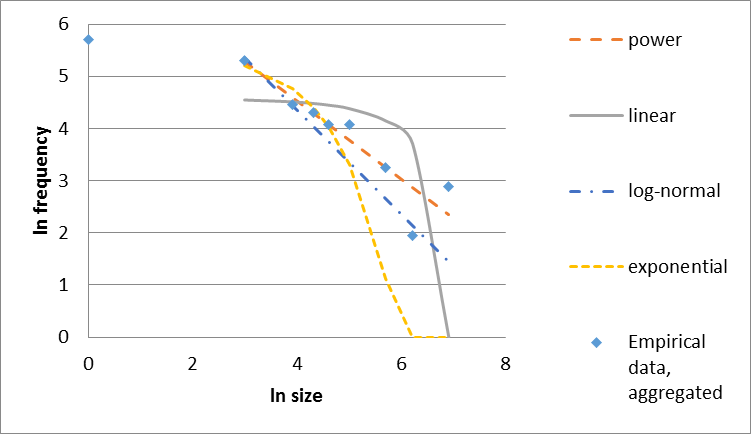
\includegraphics[width=1.0\textwidth]{bestfits}
  \caption{Log-frequency vs. log-size, with best parametric fits against aggregated data for examined distributions, minimizing sum squared error.  Note exclusion of the smallest bin (1-20) based on Hill estimation results.}
  \label{fig:bestfits}
\end{figure}

\subsection{Hill Estimation}
Figure \ref{fig:hillestimation} shows K-S statistic results from the Hill estimation technique, with fits obtained on the aggregate data using sum squared error for solver error minimization.

\begin{figure}[h]
  \centering
  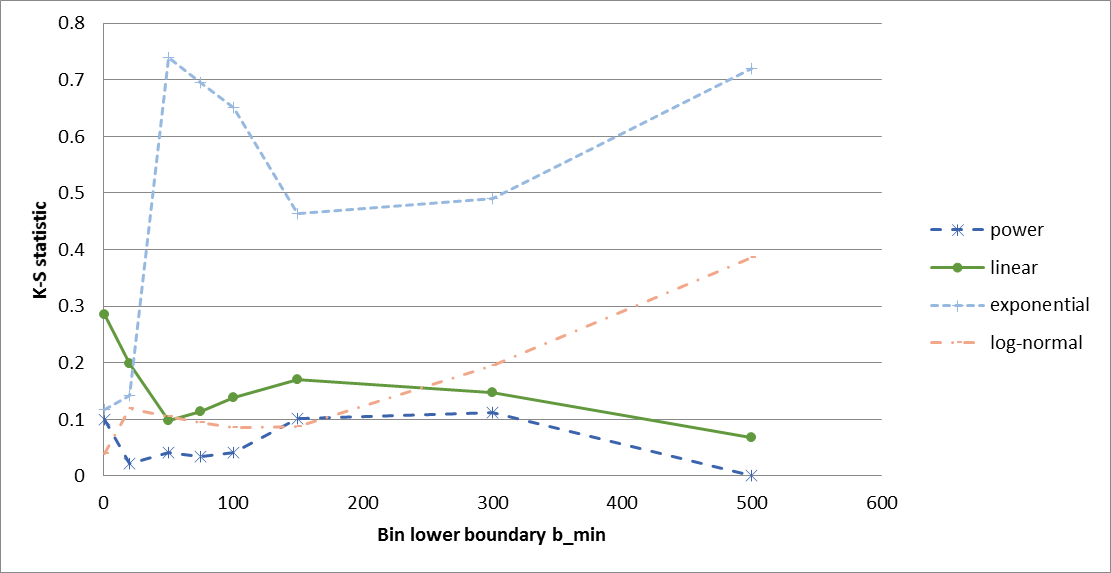
\includegraphics[width=1.0\textwidth]{hillestimation}
  \caption{Hill Estimation results on aggregate data: K-S statistics for tested distributional models to aggregated data upper tails with varying minimum bin size. The procedure reported a best (lowest) K-S statistic of 0.0222, for a power law $b_{min}$ at 20-50.}
  \label{fig:hillestimation}
\end{figure}

Hill estimating did not use bins larger than 300-500 because of proximity to the upper tail, where sampling error is more pronounced, and in any case would have eliminated most of the useful data from the analysis.

The lowest K-S statistic for the aggregate data (from among the allowed bin size choices) obtained from a power law fit with an upper tail bin lower boundary of 20 (the “20-50” size bin), using sum squared error for optimization.  The resulting power law exponent and scaling factor are $\alpha$ = 0.7463 and $C$ = 1831.5.

Hill estimation was similarly performed on the game-specific guild size distributions, with “best” (lowest K-S statistic) summarized in tabulated form in Table \ref{hillestimateresults}.

\begin{table}
	\centering
	\caption{Results of Hill estimation for specific games: best K-S, upper tail minimum bin, and distributional model for each game's guild sizes.}
	\begin{tabular}{|c r r r|}
		\hline
		 & & & best \\
		 & & best & fit \\
		Game & $b_{min}$ & K-S & \hspace{8pt} model \\ 
		\hline
		LOTRO & 20 & \hspace{8pt} 0.0374 & power \\
		\hline
		EQ2 & 100 & \hspace{8pt} 0.0268 & power \\
		\hline
		Eve & 75 & \hspace{8pt} 0.0254 & power \\
		\hline
		AoC & 150 & \hspace{8pt} 0.0183 & power \\
		\hline
		GW2 & 50 & \hspace{8pt} 0.0606 & power \\
		\hline
	\end{tabular}
	\label{hillestimateresults}
\end{table}

\section{Discussion}
The generated p-values, especially for those of the aggregate data, strongly support a power law distribution, indicating an underlying scale-invariant, complex process is involved in guild membership.
In particular for the aggregate data, the other distributions are rejected since their p-values $\ll$ 0.1 [CFN 2009].
Even visually, the power law estimate produces an astoundingly good fit with the exception of the second largest bin (500-1000) and the smallest bin (1-20).

The K-S statistics as reported by the Hill estimation technique also support this conclusion.
In the anomalous cases (AoC and Eve) where a log-normal distribution is supported over a power law, the support is weak (p-values not much higher than for a power law), or directly contradicted by alternate metrics of fitness (Hill estimation).
Additionally, it is unlikely that one game’s guild sizes would have an inherently different generative mechanism – resulting in a different distribution – than other high-membership online games.  

Of note are the low bin boundaries identified for upper-tail inclusion by the Hill estimation – in fact, in most cases the power law behavior is a remarkably better fit when the lower bins are included.
Additionally, it provides a consistently better fit over the whole range of bins examined, even if at certain minimum bin sizes it is slightly worse.
This provides more support of scale-invariant behavior, and indicates that it extends to fairly low group sizes.
Better fit with the upper tail inclusion of low bin sizes may be due to a number of factors:  higher resolution in the lower bins, and truncation in the uppermost bin. 

What the results also indicate universally is that scale invariance does not extend into the lowest bin, 1-20.
While the phenomenon of low-size nonconformance is not uncommon in the study of power law-described behavior, it is also all too commonly dismissed --- for example, as “missing” data; however, it is not apparent that explanation is justifiable here.
Gaming guilds are somewhat formalized organizations of people that group together to play games, and a large motivating factor is recruitment; as such, it is unlikely that large numbers of small guilds are under-reported.
On the other hand, there are certainly many small groups of people who play games together, who have no motivation or ability to form a formalized guild for recruitment and retention, or whose membership is too small to warrant the additional overhead and coordination costs of guild formation.
Whether or not these small informal groups constitute “missing” data is an open question, but could possibly be answered with field work to identify how many non-guild small group teams there are, and whether that data conforms to a power law model.

An insightful extension to this work would be to examine the scaling exponent and minimum bin for upper tails for guilds in various games against the frequency and types of play activities in the game.
For example, the analysis identified AoC as an outlier, having a higher minimum bin (150) for the upper tail than the other games (20 to 100).
Might this indicate a causal factor in the game itself, providing less internal guild pressure to grow beyond a certain size?
Social psychologists involved in game research or game business development might do well to investigate this.

A power law distributional model for online game guild sizes, as looks likely, might be generated by mechanisms similar to other voluntary social organizations.
As with many organizational size distributions characterized by power laws, social networks have been found to be a crucial contributing factor.
\parencite{liljeros2008} describes a simulation model that exhibits scale-free characteristics due to clustered propagation processes.
The well-known \parencite{BA1999} paper shows that growth and preferential attachment are sufficient to produce scale-free social network degree distribution.
If social networks are the driving force behind the size of social groupings – including voluntary organizations such as online gaming guilds – and if social networks exhibit power law size, then it is not surprising to find that social institutions also exhibit power law size.

While \parencite{BA1999} provide a strong causal argument for the creation of a scale-free network architecture, what is lacking generally in the literature is a single model that accounts for – and maintains, in the presence of natural growth and attrition processes – the power law distributional aspects of social organizations in the upper tail while modeling the flattening of the lower tail.
Such a model would be a rich study for future work.

\section{Conclusion}
The methods of CSN 2009 and VC 2014 were applied, with slight modification, to identify the best candidate distributional model for MMO game guild sizes.
Sum squared error was used for parametric estimation of the candidate distributions (power, linear, exponential, and log-normal). 
In most cases, a power law model was found to be the best fit to the empirical data for individual games, and was a clear best fit for the aggregate data, other distributional models being rejected for the aggregate data based on p-value analysis results.
Hill estimation was used to determine the most likely valid range of the upper tail, and also reported power law as the most likely distributional model.

Strong support for a Type II (absolute frequency) power law distributional model of MMO guild sizes indicates that scale-invariant social dynamics are generating and maintaining participation in\\guilds.
Social scientists with an interest in MMO game research and development could analyze the scaling exponent and minimum bin size for individual games to help identify potential causal differences stemming from game play.
Finally, these results indicate that scale-invariant social dynamics extend to sociality in virtual worlds --- as might be expected; further related work on distributional analysis of virtual presence in other types of online social organizations would add to the body of knowledge, and could contribute to the formation of a general complexity theory for our social life, virtual or otherwise.

\printbibliography


\end{document}